\documentclass[]{elsarticle} %review=doublespace preprint=single 5p=2 column
%%% Begin My package additions %%%%%%%%%%%%%%%%%%%
\usepackage[hyphens]{url}

  \journal{BioR\(\chi\)iv} % Sets Journal name


\usepackage{lineno} % add

\usepackage{graphicx}
%%%%%%%%%%%%%%%% end my additions to header

\usepackage[T1]{fontenc}
\usepackage{lmodern}
\usepackage{amssymb,amsmath}
\usepackage{ifxetex,ifluatex}
\usepackage{fixltx2e} % provides \textsubscript
% use upquote if available, for straight quotes in verbatim environments
\IfFileExists{upquote.sty}{\usepackage{upquote}}{}
\ifnum 0\ifxetex 1\fi\ifluatex 1\fi=0 % if pdftex
  \usepackage[utf8]{inputenc}
\else % if luatex or xelatex
  \usepackage{fontspec}
  \ifxetex
    \usepackage{xltxtra,xunicode}
  \fi
  \defaultfontfeatures{Mapping=tex-text,Scale=MatchLowercase}
  \newcommand{\euro}{€}
\fi
% use microtype if available
\IfFileExists{microtype.sty}{\usepackage{microtype}}{}
\usepackage[margin=1in]{geometry}
\bibliographystyle{elsarticle-harv}
\ifxetex
  \usepackage[setpagesize=false, % page size defined by xetex
              unicode=false, % unicode breaks when used with xetex
              xetex]{hyperref}
\else
  \usepackage[unicode=true]{hyperref}
\fi
\hypersetup{breaklinks=true,
            bookmarks=true,
            pdfauthor={},
            pdftitle={Measurement error associated with gait cycle selection in treadmill running at various speeds},
            colorlinks=false,
            urlcolor=blue,
            linkcolor=magenta,
            pdfborder={0 0 0}}
\urlstyle{same}  % don't use monospace font for urls

\setcounter{secnumdepth}{0}
% Pandoc toggle for numbering sections (defaults to be off)
\setcounter{secnumdepth}{0}


% tightlist command for lists without linebreak
\providecommand{\tightlist}{%
  \setlength{\itemsep}{0pt}\setlength{\parskip}{0pt}}


% Pandoc citation processing
\newlength{\cslhangindent}
\setlength{\cslhangindent}{1.5em}
\newlength{\csllabelwidth}
\setlength{\csllabelwidth}{3em}
\newlength{\cslentryspacingunit} % times entry-spacing
\setlength{\cslentryspacingunit}{\parskip}
% for Pandoc 2.8 to 2.10.1
\newenvironment{cslreferences}%
  {}%
  {\par}
% For Pandoc 2.11+
\newenvironment{CSLReferences}[2] % #1 hanging-ident, #2 entry spacing
 {% don't indent paragraphs
  \setlength{\parindent}{0pt}
  % turn on hanging indent if param 1 is 1
  \ifodd #1
  \let\oldpar\par
  \def\par{\hangindent=\cslhangindent\oldpar}
  \fi
  % set entry spacing
  \setlength{\parskip}{#2\cslentryspacingunit}
 }%
 {}
\usepackage{calc}
\newcommand{\CSLBlock}[1]{#1\hfill\break}
\newcommand{\CSLLeftMargin}[1]{\parbox[t]{\csllabelwidth}{#1}}
\newcommand{\CSLRightInline}[1]{\parbox[t]{\linewidth - \csllabelwidth}{#1}\break}
\newcommand{\CSLIndent}[1]{\hspace{\cslhangindent}#1}




\begin{document}


\begin{frontmatter}

  \title{Measurement error associated with gait cycle selection in
treadmill running at various speeds}
    \author[Centre for Sport Research]{Aaron S. Fox\corref{1}}
  
    \author[Centre for Sport Research]{Jason Bonacci}
  
    \author[UNSW]{John Warmenhoven}
  
    \author[Centre for Sport Research]{Meghan F. Keast}
  
      \address[Centre for Sport Research]{Centre for Sport Research,
School of Exercise and Nutrition Sciences, Deakin University, Geelong,
Australia}
    \address[UNSW]{School of Engineering and Information Technology,
University of New South Wales, Canberra, Australia}
      \cortext[1]{Corresponding Author: aaron.f@deakin.edu.au}
  
  \begin{abstract}
  A common approach in biomechanical analysis of running technique is to
  average data from several gait cycles to compute a `representative
  mean.' However, the impact of the quantity and selection of gait
  cycles on biomechanical measures is not well understood. We examined
  the effects of gait cycle selection on kinematic data by: (i)
  comparing representative means calculated from varying numbers of gait
  cycles to `global' means from the entire capture period; and (ii)
  comparing representative means from varying numbers of gait cycles
  sampled from different parts of the capture period. We used a public
  dataset (\emph{n} = 28) of lower limb kinematics captured during a
  30-second period of treadmill running at three speeds
  (2.5m·s\textsuperscript{-1}, 3.5m·s\textsuperscript{-1} and
  4.5m·s\textsuperscript{-1}). `Ground truth' values were determined by
  averaging data across all collected strides and compared to
  representative means calculated from random samples (1,000 samples) of
  \emph{n} (range = 5---30) consecutive gait cycles. We also compared
  representative means calculated from n (range = 5---15) consecutive
  gait cycles randomly sampled (1,000 samples) from within the same data
  capture period. The mean, variance and range of the absolute error of
  the representative mean compared to the `ground truth' mean
  progressively reduced across all speeds as the number of gait cycles
  used increased. Similar magnitudes of `error' were observed between
  the 2.5m·s\textsuperscript{-1} and 3.5m·s\textsuperscript{-1} speeds
  at comparable gait cycle numbers --- where the maximum errors were
  \textless{} 1.5 degrees even with a small number of gait cycles
  (i.e.~5-10). At the 4.5m·s\textsuperscript{-1} speed, maximum errors
  typically exceeded 2-4 degrees when a lower number of gait cycles were
  used. Subsequently, a higher number of gait cycles (i.e.~25-30) was
  required to achieve low errors (i.e.~1-2 degrees) at the
  4.5m·s\textsuperscript{-1} speed. The mean, variance and range of
  absolute error of representative means calculated from different parts
  of the capture period was consistent irrespective of the number of
  gait cycles used. The error between representative means was low
  (i.e.~\textless{} 1.5 degrees) and consistent across the different
  number of gait cycles at the 2.5m·s\textsuperscript{-1} and
  3.5m·s\textsuperscript{-1} speeds, and consistent but larger (i.e.~up
  to 2-4 degrees) at the 4.5m·s\textsuperscript{-1} speed. Our findings
  suggest that selecting as many gait cycles as possible from a
  treadmill running bout will minimise potential `error.' Analysing a
  small sample (i.e.~5-10 cycles) will typically result in minimal
  `error' (i.e.~\textless{} 2 degrees), particularly at lower speeds
  (i.e.~2.5m·s\textsuperscript{-1} and 3.5m·s\textsuperscript{-1}).
  Researchers and clinicians should consider the balance between
  practicalities of collecting and analysing a smaller number of gait
  cycles against the potential `error' when determining their
  methodological approach. Irrespective of the number of gait cycles
  used, we recommend that the potential `error' introduced by the choice
  of gait cycle number be considered when interpreting the magnitude of
  effects in treadmill-based running studies.
  \end{abstract}
  
 \end{frontmatter}

\hypertarget{introduction}{%
\section{Introduction}\label{introduction}}

Collecting and analysing biomechanical data is frequently used to
examine running technique. A common methodological approach is to
average data from several gait cycles to compute a given biomechanical
measure. Calculating this `representative mean' is thought to be
representative of the individuals broader running technique. Given the
inherent variability in human movement {[}1{]}, the quantity and
selection of gait cycles used to create this `representative mean'
appears an important choice in accurately quantifying an individuals
running gait. However, the number of gait cycles used in biomechanical
studies of running varies across the literature {[}2{]}. Further, very
rarely (if ever) is the decision process underpinning the quantity and
selection of gait cycles explained.

~

It is possible to collect a large number of gait cycles during
biomechanical testing, especially during treadmill running. Enabling a
participant to settle into a steady gait rhythm may better represent a
habitual running pattern. While the collection of a large number of gait
cycles can be relatively easy, it is important to give consideration to
the analysis of this data. Inflated data cleaning (e.g.~labelling and
gap filling motion capture data) and analysis (e.g.~processing frames
via inverse kinematics) time occur when processing a running trial that
uses many gait cycles. Similarly, trials with many gait cycles require
greater data storage access due to larger file sizes. An additional
consideration is which gait cycles are selected from within a capture
period. Studies often perform an extended capture period where
additional gait cycles are collected around those used for analysis
(e.g. {[}4{]}). The impact of this gait cycle selection on biomechanical
outcome measures is yet to be investigated. Better understanding of the
impact of gait cycle selection on biomechanical outcome measures may
help optimise data collection and analysis practices.

~

Oliveira and Pirscoveanu {[}2{]} examined the typical number of gait
cycles used in running biomechanics studies. On average, 12 gait cycles
were used to generate biomechanical outcome measures, though very few of
these studies (5 out of 56) used more than 10 cycles {[}2{]}. The impact
of sample size (i.e.~10 to 40 runners) and number of gait cycles (i.e.~5
to 40 steps) used on biomechanical outcome measures (i.e.~foot contact
time, loading rate, peak vertical ground reaction force, peak braking
force, running speed, and foot contact angle) was also examined {[}2{]}.
The authors found that greater than 10 strides are typically required to
achieve stable biomechanical measures in runners and collecting at least
25 strides will increase the likelihood of achieving stability in the
range of biomechanical measures examined {[}2{]}. These findings are
specific to overground running and the set of biomechanical measures
analysed. Treadmill running is often used in research {[}5{]}, and it is
plausible that the required number of gait cycles required to achieve
stability may be different to overground running. Further, Oliveira and
Pirscoveanu {[}2{]} did not examine lower limb kinematic variables
commonly reported in gait biomechanics studies. These kinematic
variables can be presented as both `zero-dimensional' (0D; e.g.~peak
values) and `one-dimensional' (1D; e.g.~time-normalised kinematic
waveform) variables {[}6{]}. Analyses of these common kinematic
variables in both their 0D and 1D forms may provide valuable insight
into the number of gait cycles required in biomechanical research.
Lastly, Oliveira and Pirscoveanu's {[}2{]} analyses were driven by
understanding data stability and statistical significance between two
running conditions (i.e.~`normal' vs.~`silent' running). A different
approach focused on understanding the magnitude of `error' introduced by
analysing different numbers of gait cycles can further our understanding
of how gait cycle selection practices impact biomechanical outcome
measures. Specifically, understanding the potential `error' introduced
by selecting a different number of gait cycles can aid in interpreting
the legitimacy of an effect (i.e.~could small effects be due to the set
of gait cycles selected).

~

We sought to extend our current understanding of how the quantity and
selection of gait cycles impact lower limb kinematic measures from a
30-second data capture period of treadmill running. First, we examined
the magnitude of `error' introduced in the representative mean compared
to the entire bout of treadmill running when the number of gait cycle
samples is varied. Second, we examined the potential variation
introduced in the representative mean when sampling a set number of gait
cycles from different parts of the capture period.

\hypertarget{methods}{%
\section{Methods}\label{methods}}

\hypertarget{dataset}{%
\subsection{Dataset}\label{dataset}}

~

We used the public dataset of treadmill running biomechanics from
Fukuchi et al. {[}7{]}. The specifics of this dataset can be found in
the associated paper {[}7{]}. Briefly, this dataset contains
lower-extremity kinematics and kinetics of 28 regular runners (27 male,
1 female; age = 34.8 ± 6.7 years; height = 176.0 ± 6.8 cm; mass = 69.6 ±
7.7 kg; running experience = 8.5 ± 7.0 years; running pace = 4.1 ± 0.4
min/km) {[}7{]}. Running kinematics were collected using a 12-camera 3D
motion capture system (Raptor-4, Motion Analysis, Santa Rosa, CA, United
States) and ground reaction force (GRF) data via an instrumented
dual-belt treadmill (FIT, Bertec, Columbus, OH, United States) {[}7{]}.
Participants ran on the treadmill at three speeds in order
(2.5m·s\textsuperscript{-1}, 3.5m·s\textsuperscript{-1} and
4.5m·s\textsuperscript{-1}), during which a three-minute accommodation
period was provided followed by a 30-second data collection period
{[}7{]}.

~

We processed the raw experimental data from Fukuchi et al. {[}7{]} using
OpenSim 4.0 {[}8{]}. Segment geometry of a generic musculoskeletal model
of the pelvis and lower limb provided by Lai et al. {[}9{]} were scaled
for each participant using their static calibration trial, which was
also used as a reference for adjusting marker positions on the model.
Lower limb joint angles were calculated using filtered (10Hz low-pass
4\textsuperscript{th} order Butterworth) marker trajectory data within
inverse kinematics analysis. GRF data were filtered using the same
cut-off frequency and filter. The filtering procedures reflected those
originally performed by Fukuchi et al. {[}7{]}. Foot strike and toe-off
events were determined when the vertical GRF crossed a 20N threshold,
also in line with the original work {[}7{]}.

\hypertarget{data-analysis}{%
\subsection{Data Analysis}\label{data-analysis}}

~

Kinematic variables common to gait biomechanics studies (i.e.~hip
flexion/extension, hip adduction/abduction, hip internal/external
rotation, knee flexion and ankle plantarflexion/dorsiflexion) were
extracted from the right limb for all participants. Data between
consecutive foot strikes were extracted and time-normalised to 0-100\%
of the gait cycle. The time-normalised 1D curves were used in subsequent
1D analyses, while a set of peak variables (hip flexion, hip adduction,
hip internal rotation, knee flexion, ankle dorsiflexion) were calculated
and extracted for the 0D analyses.

~

To examine how the number of gait cycles used impacts the representative
kinematic mean (i.e.~aim 1), we determined `ground truth' values to
compare to for the 0D and 1D kinematic variables by calculating the mean
from all available gait cycles in the 30-second capture period of
treadmill running. This value was thought to be the `most
representative' of each participants average running kinematics and was
not influenced by the selection of a subset of gait cycles. We then
iteratively calculated mean values across the kinematic variables using
a range (\emph{n} = 5 --- 30) of gait cycles from the data capture
period. For each iteration, a random sample of \emph{n} consecutive gait
cycles were extracted and used to calculate a representative kinematic
mean. We then compared this representative kinematic mean to the `ground
truth' value for the respective variable to determine the `error' that
gait cycle number selection could introduce.

~

To examine how sampling gait cycles from different sections of the
capture period impacts the representative kinematic mean (i.e.~aim 2),
we iteratively calculated representative kinematic means using a range
(\emph{n} = 5 --- 15) of randomly sampled consecutive gait cycles from
different parts of the capture period. A smaller range of gait cycles
was required for this analysis to avoid sharing gait cycles between the
calculated means. For each sampling iteration, we randomly sampled
\emph{n} consecutive gait cycles from two non-overlapping parts of the
capture period. We then compared the calculated representative kinematic
means between the two parts to determine the `error' or variation that
selection of gait cycles from different parts of the capture period
could introduce.

~

We quantified `error' in a similar fashion across both aims. For 0D
variables, the absolute difference between the representative mean and
`ground truth' (i.e.~aim 1) or two representative means (i.e.~aim 2) was
recorded in each sampling iteration. For 1D variables, the absolute
difference between the representative mean and `ground truth' (i.e.~aim
1) or two representative means (i.e.~aim 2) at each point across the
time-normalised gait cycle were calculated, and the peak difference
recorded. The random sampling process for each \emph{n} of gait cycles
was repeated 1,000 times for each participant at each running speed ---
and the `error' values collated to present descriptive statistics
(i.e.~mean ± standard deviation {[}SD{]}, median, range, inter-quartile
range) for each gait cycle number across the kinematic variables and
running speeds.

\newpage

\hypertarget{results}{%
\section{Results}\label{results}}

\hypertarget{how-does-the-number-of-gait-cycles-used-impact-the-representative-kinematic-mean}{%
\subsection{How does the number of gait cycles used impact the
representative kinematic
mean?}\label{how-does-the-number-of-gait-cycles-used-impact-the-representative-kinematic-mean}}

~

For the peak 0D kinematic variables, the mean, variance and range of the
absolute error of the representative kinematic mean compared to the
`ground truth' mean progressively reduced as the number of gait cycles
used increased (see Figures \ref{fig:groundTruthError-runT25-0D},
\ref{fig:groundTruthError-runT35-0D} and
\ref{fig:groundTruthError-runT45-0D}). Similar magnitudes of `error'
were observed between the 2.5m·s\textsuperscript{-1} and
3.5m·s\textsuperscript{-1} speeds across the 0D kinematic variables at
comparable gait cycle numbers --- where the maximum errors were less
than 1 degree even when using a small number of gait cycles. The maximum
errors at the 4.5m·s\textsuperscript{-1} speed typically exceeded 1-2
degrees, particularly for peak hip and knee joint angles when a lower
number of gait cycles were used. Subsequently, a much higher number of
gait cycles (i.e.~25-30) were required at 4.5m·s\textsuperscript{-1} to
achieve a similar magnitude of error seen at the slower running speeds.
The larger `error' values observed at 4.5m·s\textsuperscript{-1} were
driven by a bimodal distribution --- whereby certain sampling iterations
within the same biomechanical measure could produce relatively higher
versus lower errors (see Figure \ref{fig:groundTruthError-runT45-0D}).
The exception to this difference at the higher speed was for peak ankle
dorsiflexion, where similarly low `error' values and ranges
(i.e.~\textless{} 0.5 degrees) were observed across all speeds.

~

\begin{figure}

{\centering \includegraphics[width=1\linewidth]{D:/+GitRepos+/biomech-trial-selection/Analysis/GroundTruthComp/Figures/AbsoluteError_NoGaitCycle_runT25_0D} 

}

\caption{Absolute error in peak kinematic variables (i.e. zero-dimensional [0D]) when running at 2.5m·s$^{-1}$ using a subset of gait cycles versus all gait cycles from the 30-second treadmill bout. Darker points and solid lines equate to the mean ± standard deviation. Horizontal lines within boxes equate to the median value, boxes indicate the 25$^{th}$ to 75$^{th}$ percentile, and dashed whiskers indicate the range. Shaded violins are included to illustrate the distribution of values. FLEX — flexion; EXT — extension; ADD — adduction; ABD — abduction; IR — internal rotation; ER — external rotation; DF — dorsiflexion; PF — plantarflexion.}\label{fig:groundTruthError-runT25-0D}
\end{figure}

\begin{figure}

{\centering \includegraphics[width=1\linewidth]{D:/+GitRepos+/biomech-trial-selection/Analysis/GroundTruthComp/Figures/AbsoluteError_NoGaitCycle_runT35_0D} 

}

\caption{Absolute error in peak kinematic variables (i.e. zero-dimensional [0D]) when running at 3.5m·s$^{-1}$ using a subset of gait cycles versus all gait cycles from the 30-second treadmill bout. Darker points and solid lines equate to the mean ± standard deviation. Horizontal lines within boxes equate to the median value, boxes indicate the 25$^{th}$ to 75$^{th}$ percentile, and dashed whiskers indicate the range. Shaded violins are included to illustrate the distribution of values. FLEX — flexion; EXT — extension; ADD — adduction; ABD — abduction; IR — internal rotation; ER — external rotation; DF — dorsiflexion; PF — plantarflexion.}\label{fig:groundTruthError-runT35-0D}
\end{figure}

\begin{figure}

{\centering \includegraphics[width=1\linewidth]{D:/+GitRepos+/biomech-trial-selection/Analysis/GroundTruthComp/Figures/AbsoluteError_NoGaitCycle_runT45_0D} 

}

\caption{Absolute error in peak kinematic variables (i.e. zero-dimensional [0D]) when running at 4.5m·s$^{-1}$ using a subset of gait cycles versus all gait cycles from the 30-second treadmill bout. Darker points and solid lines equate to the mean ± standard deviation. Horizontal lines within boxes equate to the median value, boxes indicate the 25$^{th}$ to 75$^{th}$ percentile, and dashed whiskers indicate the range. Shaded violins are included to illustrate the distribution of values. FLEX — flexion; EXT — extension; ADD — adduction; ABD — abduction; IR — internal rotation; ER — external rotation; DF — dorsiflexion; PF — plantarflexion.}\label{fig:groundTruthError-runT45-0D}
\end{figure}

We observed near identical characteristics of the mean, variance and
range of the peak absolute error of the representative kinematic mean
compared to the mean from all gait cycles for the 1D kinematic variables
(see Figures \ref{fig:groundTruthError-runT25-1D},
\ref{fig:groundTruthError-runT35-1D} and
\ref{fig:groundTruthError-runT45-1D}). As with the 0D variables, the
potential `error' reduced as the number of gait cycles increased, and
similarly low magnitudes of `error' (i.e.~\textless{} 1 degree) were at
the 2.5m·s\textsuperscript{-1} and 3.5m·s\textsuperscript{-1} speeds.
Larger `errors' exceeding 1-2 degrees with lower gait cycle numbers were
present at the 4.5m·s\textsuperscript{-1} speed (with the exception of
ankle dorsi/plantarflexion), with this again driven by a more bimodal
distribution of samples (see Figure
\ref{fig:groundTruthError-runT45-1D}).

~

\begin{figure}

{\centering \includegraphics[width=1\linewidth]{D:/+GitRepos+/biomech-trial-selection/Analysis/GroundTruthComp/Figures/AbsoluteError_NoGaitCycle_runT25_1D} 

}

\caption{Peak absolute error in kinematic variables across the gait cycle (i.e. one-dimensional [1D]) when running at 2.5m·s$^{-1}$ using a subset of gait cycles versus all gait cycles from the 30-second treadmill bout. Darker points and solid lines equate to the mean ± standard deviation. Horizontal lines within boxes equate to the median value, boxes indicate the 25$^{th}$ to 75$^{th}$ percentile, and dashed whiskers indicate the range. Shaded violins are included to illustrate the distribution of values. FLEX — flexion; EXT — extension; ADD — adduction; ABD — abduction; IR — internal rotation; ER — external rotation; DF — dorsiflexion; PF — plantarflexion.}\label{fig:groundTruthError-runT25-1D}
\end{figure}

\begin{figure}

{\centering \includegraphics[width=1\linewidth]{D:/+GitRepos+/biomech-trial-selection/Analysis/GroundTruthComp/Figures/AbsoluteError_NoGaitCycle_runT35_1D} 

}

\caption{Peak absolute error in kinematic variables across the gait cycle (i.e. one-dimensional [1D]) when running at 3.5m·s$^{-1}$ using a subset of gait cycles versus all gait cycles from the 30-second treadmill bout. Darker points and solid lines equate to the mean ± standard deviation. Horizontal lines within boxes equate to the median value, boxes indicate the 25$^{th}$ to 75$^{th}$ percentile, and dashed whiskers indicate the range. Shaded violins are included to illustrate the distribution of values. FLEX — flexion; EXT — extension; ADD — adduction; ABD — abduction; IR — internal rotation; ER — external rotation; DF — dorsiflexion; PF — plantarflexion.}\label{fig:groundTruthError-runT35-1D}
\end{figure}

\begin{figure}

{\centering \includegraphics[width=1\linewidth]{D:/+GitRepos+/biomech-trial-selection/Analysis/GroundTruthComp/Figures/AbsoluteError_NoGaitCycle_runT45_1D} 

}

\caption{Peak absolute error in kinematic variables across the gait cycle (i.e. one-dimensional [1D]) when running at 4.5m·s$^{-1}$ using a subset of gait cycles versus all gait cycles from the 30-second treadmill bout. Darker points and solid lines equate to the mean ± standard deviation. Horizontal lines within boxes equate to the median value, boxes indicate the 25$^{th}$ to 75$^{th}$ percentile, and dashed whiskers indicate the range. Shaded violins are included to illustrate the distribution of values. FLEX — flexion; EXT — extension; ADD — adduction; ABD — abduction; IR — internal rotation; ER — external rotation; DF — dorsiflexion; PF — plantarflexion.}\label{fig:groundTruthError-runT45-1D}
\end{figure}

\hypertarget{how-does-the-selection-of-gait-cycles-impact-the-representative-kinematic-mean}{%
\subsection{How does the selection of gait cycles impact the
representative kinematic
mean?}\label{how-does-the-selection-of-gait-cycles-impact-the-representative-kinematic-mean}}

~

The mean, variance and range of the absolute error (or variation) of the
representative kinematic mean compared to the mean from all gait cycles
for the peak 0D kinematic variables remained relatively consistent
irrespective of the number of gait cycles used when sampling from
different parts of the capture period (see Figures
\ref{fig:samplesComp-runT25-0D}, \ref{fig:samplesComp-runT35-0D} and
\ref{fig:samplesComp-runT45-0D}). At the 2.5m·s\textsuperscript{-1} and
3.5m·s\textsuperscript{-1} speeds, the variation in peak kinematic
variables was always less than 1.5 degrees. However, peak knee flexion
had the potential for larger variation compared to the remaining
kinematic variables (see Figures \ref{fig:samplesComp-runT25-0D} and
\ref{fig:samplesComp-runT35-0D}). While the potential variation between
gait cycle samples was consistent with increasing gait cycle numbers at
the 4.5m·s\textsuperscript{-1} speed, a higher mean and range of
potential variation (i.e.~up to 2-4 degrees) was evident across the peak
kinematic variables (with the exception of peak ankle dorsiflexion). As
in the previous analyses, we observed a bimodal distribution of the
samples at the 4.5m·s\textsuperscript{-1} speed (see Figure
\ref{fig:samplesComp-runT45-0D}).

~

\begin{figure}

{\centering \includegraphics[width=1\linewidth]{D:/+GitRepos+/biomech-trial-selection/Analysis/SamplesComp/Figures/AbsoluteError_NoGaitCycle_runT25_0D} 

}

\caption{Absolute error in peak kinematic variables (i.e. zero-dimensional [0D]) when running at 2.5m·s$^{-1}$ using a two comparative subsets of gait cycles from the 30-second treadmill bout. Darker points and solid lines equate to the mean ± standard deviation. Horizontal lines within boxes equate to the median value, boxes indicate the 25$^{th}$ to 75$^{th}$ percentile, and dashed whiskers indicate the range. Shaded violins are included to illustrate the distribution of values. FLEX — flexion; EXT — extension; ADD — adduction; ABD — abduction; IR — internal rotation; ER — external rotation; DF — dorsiflexion; PF — plantarflexion.}\label{fig:samplesComp-runT25-0D}
\end{figure}

\begin{figure}

{\centering \includegraphics[width=1\linewidth]{D:/+GitRepos+/biomech-trial-selection/Analysis/SamplesComp/Figures/AbsoluteError_NoGaitCycle_runT35_0D} 

}

\caption{Absolute error in peak kinematic variables (i.e. zero-dimensional [0D]) when running at 3.5m·s$^{-1}$ using a two comparative subsets of gait cycles from the 30-second treadmill bout. Darker points and solid lines equate to the mean ± standard deviation. Horizontal lines within boxes equate to the median value, boxes indicate the 25$^{th}$ to 75$^{th}$ percentile, and dashed whiskers indicate the range. Shaded violins are included to illustrate the distribution of values. FLEX — flexion; EXT — extension; ADD — adduction; ABD — abduction; IR — internal rotation; ER — external rotation; DF — dorsiflexion; PF — plantarflexion.}\label{fig:samplesComp-runT35-0D}
\end{figure}

\begin{figure}

{\centering \includegraphics[width=1\linewidth]{D:/+GitRepos+/biomech-trial-selection/Analysis/SamplesComp/Figures/AbsoluteError_NoGaitCycle_runT45_0D} 

}

\caption{Absolute error in peak kinematic variables (i.e. zero-dimensional [0D]) when running at 4.5m·s$^{-1}$ using a two comparative subsets of gait cycles from the 30-second treadmill bout. Darker points and solid lines equate to the mean ± standard deviation. Horizontal lines within boxes equate to the median value, boxes indicate the 25$^{th}$ to 75$^{th}$ percentile, and dashed whiskers indicate the range. Shaded violins are included to illustrate the distribution of values. FLEX — flexion; EXT — extension; ADD — adduction; ABD — abduction; IR — internal rotation; ER — external rotation; DF — dorsiflexion; PF — plantarflexion.}\label{fig:samplesComp-runT45-0D}
\end{figure}

We observed similar characteristics for the mean, variance and range of
the absolute error (or variation) of the representative kinematic mean
compared to the mean from all gait cycles for the 1D kinematic variables
when sampling gait cycles from different parts of the capture period
(see Figures \ref{fig:samplesComp-runT25-1D},
\ref{fig:samplesComp-runT35-1D} and \ref{fig:samplesComp-runT45-1D}).
The potential variation remained low (i.e.~\textless{} 1.5 degrees) and
consistent across the different number of gait cycles at the
2.5m·s\textsuperscript{-1} and 3.5m·s\textsuperscript{-1} speeds (see
Figures \ref{fig:samplesComp-runT25-1D} and
\ref{fig:samplesComp-runT35-1D}). The potential variation remained
consistent but increased in magnitude (i.e.~up to 2-4 degrees), and
shifted to a bimodal distribution at the 4.5m·s\textsuperscript{-1}
speed (see Figure \ref{fig:samplesComp-runT45-1D}). In contrast to the
0D variables, this shift was evident in all 1D kinematic variables
(including ankle dorsi/plantarflexion).

~

\begin{figure}

{\centering \includegraphics[width=1\linewidth]{D:/+GitRepos+/biomech-trial-selection/Analysis/SamplesComp/Figures/AbsoluteError_NoGaitCycle_runT25_1D} 

}

\caption{Peak absolute error in kinematic variables across the gait cycle (i.e. one-dimensional [1D]) when running at 2.5m·s$^{-1}$ using two comparative subsets of gait cycles from the 30-second treadmill bout. Darker points and solid lines equate to the mean ± standard deviation. Horizontal lines within boxes equate to the median value, boxes indicate the 25$^{th}$ to 75$^{th}$ percentile, and dashed whiskers indicate the range. Shaded violins are included to illustrate the distribution of values. FLEX — flexion; EXT — extension; ADD — adduction; ABD — abduction; IR — internal rotation; ER — external rotation; DF — dorsiflexion; PF — plantarflexion.}\label{fig:samplesComp-runT25-1D}
\end{figure}

\begin{figure}

{\centering \includegraphics[width=1\linewidth]{D:/+GitRepos+/biomech-trial-selection/Analysis/SamplesComp/Figures/AbsoluteError_NoGaitCycle_runT35_1D} 

}

\caption{Peak absolute error in kinematic variables across the gait cycle (i.e. one-dimensional [1D]) when running at 3.5m·s$^{-1}$ using two comparative subsets of gait cycles from the 30-second treadmill bout. Darker points and solid lines equate to the mean ± standard deviation. Horizontal lines within boxes equate to the median value, boxes indicate the 25$^{th}$ to 75$^{th}$ percentile, and dashed whiskers indicate the range. Shaded violins are included to illustrate the distribution of values. FLEX — flexion; EXT — extension; ADD — adduction; ABD — abduction; IR — internal rotation; ER — external rotation; DF — dorsiflexion; PF — plantarflexion.}\label{fig:samplesComp-runT35-1D}
\end{figure}

\begin{figure}

{\centering \includegraphics[width=1\linewidth]{D:/+GitRepos+/biomech-trial-selection/Analysis/SamplesComp/Figures/AbsoluteError_NoGaitCycle_runT45_1D} 

}

\caption{Peak absolute error in kinematic variables across the gait cycle (i.e. one-dimensional [1D]) when running at 4.5m·s$^{-1}$ using two comparative subsets of gait cycles from the 30-second treadmill bout. Darker points and solid lines equate to the mean ± standard deviation. Horizontal lines within boxes equate to the median value, boxes indicate the 25$^{th}$ to 75$^{th}$ percentile, and dashed whiskers indicate the range. Shaded violins are included to illustrate the distribution of values. FLEX — flexion; EXT — extension; ADD — adduction; ABD — abduction; IR — internal rotation; ER — external rotation; DF — dorsiflexion; PF — plantarflexion.}\label{fig:samplesComp-runT45-1D}
\end{figure}

\newpage

\hypertarget{discussion}{%
\section{Discussion}\label{discussion}}

Biomechanical studies of running often use a subset of gait cycles from
a running bout or capture period, and average across these cycles to
calculate an individual's representative mean. We examined the impact of
the quantity and selection of gait cycles from within the a capture
period on the magnitude of `error' in lower limb kinematic measures
during a continuous bout of treadmill running. We found that including a
greater number of gait cycles to calculate the representative kinematic
mean reduces the magnitude and range of potential `error.' The potential
error using a small number of gait cycles (i.e.~\emph{n} = 5-10) was low
(i.e.~typically \textless{} 1 degree) when running at
2.5m·s\textsuperscript{-1} and 3.5m·s\textsuperscript{-1}, and hence we
noted an effect of diminishing returns (i.e.~limited improvement in
error reduction above 5-10 gait cycles) by including more gait cycles at
these slower speeds. Using a similarly low number of gait cycles did
slightly inflate potential `error' (i.e.~1-4 degrees) when running at
4.5m·s\textsuperscript{-1}. We also found small magnitudes of `error' in
representative kinematic means across all running speeds when selecting
gait cycles from different parts of the capture period, and these
remained relatively consistent irrespective of the number of gait cycles
used.

~

We found that the `error' between the representative kinematic means and
the associated `ground truth' values progressively reduced with an
increasing number of gait cycles. Using a greater number of gait cycles
equated to using a higher proportion of data that were used to create
the `ground truth' --- hence this result is not surprising. More
noteworthy is the scale of `error' when using a reduced number of gait
cycles (i.e.~\emph{n} = 5-10) and the diminishing effect of using a
larger number (i.e.~\emph{n} \textgreater{} 15) of gait cycles. We
typically observed that the maximum `error' or variation with respect to
the `ground truth' was less than one degree, even at the lowest number
of gait cycles used when running at the 2.5m·s\textsuperscript{-1} and
3.5m·s\textsuperscript{-1}. This error increased up to three degrees at
4.5m·s\textsuperscript{-1}. Reducing the potential `error' compared to
the ground truth appeared to be the main effect of increasing the number
of gait cycles used. However, the reduction in potential error typically
plateaued and a diminished benefit observed when using above 15-20 gait
cycles. These patterns were consistent across both the 0D and 1D
kinematic data. The notion of diminishing returns above 15-20 gait
cycles contrasts with the findings of Oliveira and Pirscoveanu {[}2{]}
--- whereby data stability was not achieved in most runners using this
number of gait cycles. Clear differences between our study and this
existing work {[}2{]} were the metrics used to define `error' or
stability, the biomechanical measures analysed (i.e.~joint kinematics
vs.~mostly kinetic variables), and the use of treadmill (including a
3-minute familiarisation period) versus overground running. The latter
may represent an important distinction, whereby the familiarisation
period combined with the more continuous approach of treadmill running
led to participants settling into a more stable rhythm during the data
capture period. Forrester {[}10{]} performed a series of simulations
using a similar sequential analysis technique to Oliveira and
Pirscoveanu {[}2{]} to determine the number of trials required for
biomechanical measures with generic means and standard deviations. This
work {[}10{]} proposed that nine (± 8) trials were required to achieve
stability of the mean, which is more in line with our findings of
diminishing returns in `error' at 15-20 gait cycles. The mean and
variation of the biomechanical outcome measure being examined likely
plays a role in the potential `error.' We saw the largest potential
`errors' in hip and knee flexion when using a smaller number of gait
cycles and this is not surprising given these measures had the largest
means and standard deviations within the dataset {[}7{]}.

~

Despite the potential for diminishing returns, our data suggests that
researchers can minimise the potential `error' in representative
kinematic means by using more gait cycles. A simplistic recommendation
from our analyses would be to use as many gait cycles as possible.
However, this ignores the practical considerations of storing, cleaning
and processing larger biomechanical data files. Certain circumstances,
such as a large participant sample or timely computational measures
(e.g.~muscle forces derived from optimisation approaches), may make
using 20+ gait cycles impractical. Our recommendation is to balance the
practical considerations against the potential `error' or variation in
the data that can be tolerated. Consideration should be given to the
accuracy of the measure, or size of the effect researchers or clinicians
are interested in measuring. For example, using less than ten gait
cycles to explore a small effect (i.e.~\textless{} 1-2 degrees) in 1D
hip or knee flexion continua may be unwise, as the potential variation
in the calculated means could exceed the magnitude of the effect of
interest. Our data suggests that the smaller the expected effect or
magnitude of effect of interest, the greater number of gait cycles
necessary for the analyses.

~

We observed relatively small variations (i.e.~\textless{} 1.5 degrees)
between representative kinematic means calculated from gait cycle
samples extracted from different parts of the 2.5m·s\textsuperscript{-1}
and 3.5m·s\textsuperscript{-1} capture periods, while these slightly
increased (i.e.~2-4 degrees) when examining the
4.5m·s\textsuperscript{-1} speed. This magnitude of variation remained
consistent irrespective of the total number of gait cycles used. These
findings suggest that once the number of gait cycles used for analysis
is selected, the selection of these from within a capture period will
introduce a small, but consistent amount of `error.' The inherent
variability in human movement {[}1{]} is the likely and potentially
unavoidable cause of this variation. We randomly sampled differing
sections of the capture period as part of our analyses, and at-times
this generated near zero variation between the two representative means.
Without further inspection of our data, we cannot confirm what generated
the reduced variation --- but we hypothesise that the samples with
minimal to no variation likely stemmed from using sections of the
capture period in close proximity to one another. We also cannot
determine which section of the running bout is more representative or
`accurate,' as we only compared between samples and did not extend this
comparison to the `ground truth' values. Our data can only be used to
infer the potential magnitude of variation expected when using gait
cycles from different parts of a 30-second capture period. The magnitude
of this variation appears to be driven by the scale of the mean and
standard deviation of the measure (i.e.~kinematic measures with higher
means and standard deviations incur a greater magnitude of variation).
It is also plausible that greater variation could be seen during longer
capture periods than that used in the present study (i.e.~30-seconds) or
when comparing gait cycles from capture periods separated by a longer
time period (e.g.~two capture periods at either end of a 5+ minute
running bout). The dataset we used did not allow for these analyses to
be conducted, yet present relevant avenues for further research on this
topic. The practical implications of these findings once again relate to
the confidence we can have in measuring an effect on lower limb
kinematics during treadmill running. If our observed effect does not
exceed the typical variation seen when sampling from different parts of
the capture period, there is a possibility that the observed effect is
simply noise due to the gait cycles sampled.

~

Running at 4.5m·s\textsuperscript{-1} induced greater `error' relative
to the `ground truth' and between representative means from different
parts of the capture period compared to running at
2.5m·s\textsuperscript{-1} and 3.5m·s\textsuperscript{-1}. There are
various potential reasons for these results. Faster running speeds
induce larger means and standard deviations across kinematic variables
{[}7{]}, particularly in hip and knee flexion where more dramatic
increases in `error' were observed. We propose that the larger means and
standard deviations at higher speeds introduce a greater magnitude of
variation across gait cycles. An increase in gait speed could also be
considered a changed task constraint on the running movement {[}11{]},
and this change in constraint could have affected the role and magnitude
of variability at certain joints. Movement variability may help explain
the greater potential for `error' when sampling from different gait
cycles at different running speeds. The changed task constraint, and
greater kinematic means and standard deviations with increased running
speed {[}7{]} may engender expectations of a consistent increase in
potential `error' with increased running speed. It is therefore
surprising that the increase in `error' or variation was inconsistent,
and most evident and prominent when only when running at
4.5m·s\textsuperscript{-1} speed. Within the dataset examined,
participants ran for a three minute accommodation period at each speed,
following which data were collected over a 30 second period {[}7{]}. The
order of running conditions (i.e.~2.5m·s\textsuperscript{-1},
3.5m·s\textsuperscript{-1}, 4.5m·s\textsuperscript{-1}) was kept
consistent for each participant {[}7{]}. It is possible that these
experimental procedures (i.e.~running at the fastest speed towards the
end of the running period) could have introduced some fatigue when
running at 4.5m·s\textsuperscript{-1}. Running in a fatigued state can
increase biomechanical variability {[}13{]}, while also altering running
kinematics compared to a non-fatigued state {[}16{]}. If fatigue was
present during the final bout of running, it could have resulted in
greater kinematic variability or a change in running kinematics during
the 30 second period of data collection. Alternatively, fatigue may have
begun to set in within the final 30 seconds of the run --- potentially
inducing a change in running kinematics within the period where data
were collected. This latter explanation may explain the bimodal
distribution in `error' we observed in the 4.5m·s\textsuperscript{-1}
running bout, whereby larger `errors' may have been observed with gait
cycles from earlier versus later parts of the 30 second capture period.
Given we did not explicitly consider the sections where gait cycles were
sampled from, this notion is speculative. It should also be noted that
studies examining changes in running biomechanics with fatigue {[}16{]}
have used more intense and longer duration exercise protocols that what
participants experienced in our study. Despite the lack of understanding
around the potential mechanism, our study demonstrates a need to
consider gait cycle sampling practices when running at faster speeds,
and potentially when fatigue is present.

~

It is important to note that the measurement `error' or variation based
on gait cycle selection were small compared to other established sources
of error during biomechanical data collection and analysis {[}28{]}. The
magnitude of `error' in the present study is eclipsed by the errors or
variation introduced by soft-tissue artefact associated with
skin-mounted markers {[}20{]}, different joint coordinate systems
{[}23{]} or gait models {[}24{]}, kinematic algorithm choice {[}25{]},
tester experience {[}27{]}, or different measurement approaches
(i.e.~marker vs.~marker-less) {[}28{]}. The number of gait cycles used
for analysis is likely less important when considering the size of a
measured effect against the potential `error' or variation introduced by
other methodological decisions. Future research should also better
define practically meaningful effects for biomechanical outcome
measures. Using similar methods to those in other fields for defining
the smallest effect size of interest {[}29{]} may help inform whether
the magnitude of errors are acceptable for practical use and
interpretation.

~

Our results must be considered with respect to the limitations in our
approach. We only examined conditions where \emph{n} consecutive gait
cycles were sampled from a 30-second capture period during a continuous
bout of treadmill running at three set speeds. Different results might
be expected with non-consecutive selection of samples from the capture
period, or under different running conditions (e.g.~outdoor overground
running; slower or faster speeds). We also focused on peak and 1D
waveform data of lower limb kinematic variables. Other biomechanical
outcome measures (e.g.~joint moments, estimates of muscle activation and
forces) may incur variable magnitudes of `error' or variation with
respect to gait cycle selection. We inferred `error' via comparison to
values calculated from all gait cycles in the running bout (i.e.~our
`ground truth' value). Although we deemed this the best approach within
our study, it is important to acknowledge that these values may still
not represent the individuals exact or true running kinematics. Lastly,
we investigated kinematic measures at a univariate joint level. Our
findings are therefore not applicable to studies examining covariance or
dynamics across joints during gait.

\hypertarget{conclusions}{%
\section{Conclusions}\label{conclusions}}

We identified the range of potential `error' or variation in lower limb
kinematics associated with the quantity and selection of gait cycles
used from a data capture period of continuous treadmill running. Our
findings suggest that including as many gait cycles as possible from the
running bout will minimise `error.' However, the error associated with
only a small sample of gait cycles (i.e.~5-10 gait cycles) was typically
quite small (\textless{} 3 degrees) when running at
2.5m·s\textsuperscript{-1} and 3.5m·s\textsuperscript{-1}. Larger
potential `errors' or variation were observed when analysing kinematic
variables with larger means and standard deviations, and when running at
faster speeds (i.e.~4.5m·s\textsuperscript{-1}). Researchers and
clinicians should balance the benefits of a reduction in potential
`error' with the challenges of collecting, processing and analysing a
large number of gait cycles when determining their methodological
approach. We recommend that the potential `error' or variation
introduced by the quantity and selection of gait cycles be considered
when interpreting effects from treadmill-based running studies.
Specifically, researchers must consider the magnitude of potential
`error' against the identified effects between groups or following an
intervention.

\newpage

\hypertarget{references}{%
\section*{References}\label{references}}
\addcontentsline{toc}{section}{References}

\hypertarget{refs}{}
\begin{CSLReferences}{0}{0}
\leavevmode\vadjust pre{\hypertarget{ref-vanEmmerik2000}{}}%
\CSLLeftMargin{{[}1{]} }
\CSLRightInline{Emmerik REA van, Wegen EEH van. {On Variability and
Stability in Human Movement}. Journal of Applied Biomechanics
2000;16:394--406.
doi:\href{https://doi.org/10.1123/jab.16.4.394}{10.1123/jab.16.4.394}.}

\leavevmode\vadjust pre{\hypertarget{ref-Oliveira2021}{}}%
\CSLLeftMargin{{[}2{]} }
\CSLRightInline{Oliveira AS, Pirscoveanu CI. {Implications of sample
size and acquired number of steps to investigate running biomechanics}.
Scientific Reports 2021;11:3083.
doi:\href{https://doi.org/10.1038/s41598-021-82876-z}{10.1038/s41598-021-82876-z}.}

\leavevmode\vadjust pre{\hypertarget{ref-Fellin2010}{}}%
\CSLLeftMargin{{[}3{]} }
\CSLRightInline{Fellin RE, Manal K, Davis IS. {Comparison of lower
extremity kinematic curves during overground and treadmill running.}
Journal of Applied Biomechanics 2010;26:407--14.
doi:\href{https://doi.org/10.1126/scisignal.2001449.Engineering}{10.1126/scisignal.2001449.Engineering}.}

\leavevmode\vadjust pre{\hypertarget{ref-Fox2021}{}}%
\CSLLeftMargin{{[}4{]} }
\CSLRightInline{Fox AS, Ferber R, Bonacci J. {Kinematic and Coordination
Variability in Individuals With Acute and Chronic Patellofemoral Pain}.
Journal of Applied Biomechanics 2021;37:463--70.
doi:\href{https://doi.org/10.1123/jab.2020-0401}{10.1123/jab.2020-0401}.}

\leavevmode\vadjust pre{\hypertarget{ref-VanHooren2020}{}}%
\CSLLeftMargin{{[}5{]} }
\CSLRightInline{Van Hooren B, Fuller JT, Buckley JD, Miller JR, Sewell
K, Rao G, et al. {Is Motorized Treadmill Running Biomechanically
Comparable to Overground Running? A Systematic Review and Meta-Analysis
of Cross-Over Studies}. Sports Medicine 2020;50:785--813.
doi:\href{https://doi.org/10.1007/s40279-019-01237-z}{10.1007/s40279-019-01237-z}.}

\leavevmode\vadjust pre{\hypertarget{ref-Pataky2016}{}}%
\CSLLeftMargin{{[}6{]} }
\CSLRightInline{Pataky TC, Vanrenterghem J, Robinson MA. {The
probability of false positives in zero-dimensional analyses of
one-dimensional kinematic, force and EMG trajectories}. Journal of
Biomechanics 2016;49:1468--76.
doi:\href{https://doi.org/10.1016/j.jbiomech.2016.03.032}{10.1016/j.jbiomech.2016.03.032}.}

\leavevmode\vadjust pre{\hypertarget{ref-Fukuchi2017}{}}%
\CSLLeftMargin{{[}7{]} }
\CSLRightInline{Fukuchi RK, Fukuchi CA, Duarte M. {A public dataset of
running biomechanics and the effects of running speed on lower extremity
kinematics and kinetics}. PeerJ 2017;5:e3298.
doi:\href{https://doi.org/10.7717/peerj.3298}{10.7717/peerj.3298}.}

\leavevmode\vadjust pre{\hypertarget{ref-Delp2007}{}}%
\CSLLeftMargin{{[}8{]} }
\CSLRightInline{Delp SL, Anderson FC, Arnold AS, Loan P, Habib A, John
CT, et al. {OpenSim: Open-Source Software to Create and Analyze Dynamic
Simulations of Movement}. IEEE Transactions on Biomedical Engineering
2007;54:1940--50.
doi:\href{https://doi.org/10.1109/TBME.2007.901024}{10.1109/TBME.2007.901024}.}

\leavevmode\vadjust pre{\hypertarget{ref-Lai2017}{}}%
\CSLLeftMargin{{[}9{]} }
\CSLRightInline{Lai AKM, Arnold AS, Wakeling JM. {Why are Antagonist
Muscles Co-activated in My Simulation? A Musculoskeletal Model for
Analysing Human Locomotor Tasks}. Annals of Biomedical Engineering
2017;45:2762--74.
doi:\href{https://doi.org/10.1007/s10439-017-1920-7}{10.1007/s10439-017-1920-7}.}

\leavevmode\vadjust pre{\hypertarget{ref-Forrester2015}{}}%
\CSLLeftMargin{{[}10{]} }
\CSLRightInline{Forrester SE. {Selecting the number of trials in
experimental biomechanics studies}. International Biomechanics
2015;2:62--72.
doi:\href{https://doi.org/10.1080/23335432.2015.1049296}{10.1080/23335432.2015.1049296}.}

\leavevmode\vadjust pre{\hypertarget{ref-Newell1985}{}}%
\CSLLeftMargin{{[}11{]} }
\CSLRightInline{Newell KM. {Coordination, Control and Skill}. Advances
in Psychology 1985;27:295--317.
doi:\href{https://doi.org/10.1016/S0166-4115(08)62541-8}{10.1016/S0166-4115(08)62541-8}.}

\leavevmode\vadjust pre{\hypertarget{ref-Meardon2011}{}}%
\CSLLeftMargin{{[}12{]} }
\CSLRightInline{Meardon SA, Hamill J, Derrick TR. {Running injury and
stride time variability over a prolonged run}. Gait \& Posture
2011;33:36--40.
doi:\href{https://doi.org/10.1016/j.gaitpost.2010.09.020}{10.1016/j.gaitpost.2010.09.020}.}

\leavevmode\vadjust pre{\hypertarget{ref-Chen2022}{}}%
\CSLLeftMargin{{[}13{]} }
\CSLRightInline{Chen TL-W, Wong DW-C, Wang Y, Tan Q, Lam W-K, Zhang M.
{Changes in segment coordination variability and the impacts of the
lower limb across running mileages in half marathons: Implications for
running injuries}. Journal of Sport and Health Science 2022;11:67--74.
doi:\href{https://doi.org/10.1016/j.jshs.2020.09.006}{10.1016/j.jshs.2020.09.006}.}

\leavevmode\vadjust pre{\hypertarget{ref-BazueloRuiz2018}{}}%
\CSLLeftMargin{{[}14{]} }
\CSLRightInline{Bazuelo-Ruiz B, Durá-Gil JV, Palomares N, Medina E,
Llana-Belloch S. {Effect of fatigue and gender on kinematics and ground
reaction forces variables in recreational runners}. PeerJ 2018;6:e4489.
doi:\href{https://doi.org/10.7717/peerj.4489}{10.7717/peerj.4489}.}

\leavevmode\vadjust pre{\hypertarget{ref-Derrick2002}{}}%
\CSLLeftMargin{{[}15{]} }
\CSLRightInline{Derrick TR, Dereu D, McLean SP. {Impacts and kinematic
adjustments during an exhaustive run.} Medicine and Science in Sports
and Exercise 2002;34:998--1002.
doi:\href{https://doi.org/10.1097/00005768-200206000-00015}{10.1097/00005768-200206000-00015}.}

\leavevmode\vadjust pre{\hypertarget{ref-Mizrahi2000}{}}%
\CSLLeftMargin{{[}16{]} }
\CSLRightInline{Mizrahi J, Verbitsky O, Isakov E, Daily D. {Effect of
fatigue on leg kinematics and impact acceleration in long distance
running}. Human Movement Science 2000;19:139--51.
doi:\href{https://doi.org/10.1016/S0167-9457(00)00013-0}{10.1016/S0167-9457(00)00013-0}.}

\leavevmode\vadjust pre{\hypertarget{ref-Leardini2005}{}}%
\CSLLeftMargin{{[}17{]} }
\CSLRightInline{Leardini A, Chiari L, Croce UD, Cappozzo A. {Human
movement analysis using stereophotogrammetry}. Gait \& Posture
2005;21:212--25.
doi:\href{https://doi.org/10.1016/j.gaitpost.2004.05.002}{10.1016/j.gaitpost.2004.05.002}.}

\leavevmode\vadjust pre{\hypertarget{ref-Benoit2015}{}}%
\CSLLeftMargin{{[}18{]} }
\CSLRightInline{Benoit DL, Damsgaard M, Andersen MS. {Surface marker
cluster translation, rotation, scaling and deformation: Their
contribution to soft tissue artefact and impact on knee joint
kinematics}. Journal of Biomechanics 2015;48:2124--9.
doi:\href{https://doi.org/10.1016/j.jbiomech.2015.02.050}{10.1016/j.jbiomech.2015.02.050}.}

\leavevmode\vadjust pre{\hypertarget{ref-Fiorentino2017}{}}%
\CSLLeftMargin{{[}19{]} }
\CSLRightInline{Fiorentino NM, Atkins PR, Kutschke MJ, Goebel JM,
Foreman KB, Anderson AE. {Soft tissue artifact causes significant errors
in the calculation of joint angles and range of motion at the hip}. Gait
\& Posture 2017;55:184--90.
doi:\href{https://doi.org/10.1016/j.gaitpost.2017.03.033}{10.1016/j.gaitpost.2017.03.033}.}

\leavevmode\vadjust pre{\hypertarget{ref-DIsidoro2020}{}}%
\CSLLeftMargin{{[}20{]} }
\CSLRightInline{D'Isidoro F, Brockmann C, Ferguson SJ. {Effects of the
soft tissue artefact on the hip joint kinematics during unrestricted
activities of daily living}. Journal of Biomechanics 2020;104:109717.
doi:\href{https://doi.org/10.1016/j.jbiomech.2020.109717}{10.1016/j.jbiomech.2020.109717}.}

\leavevmode\vadjust pre{\hypertarget{ref-Baudet2014}{}}%
\CSLLeftMargin{{[}21{]} }
\CSLRightInline{Baudet A, Morisset C, D'Athis P, Maillefert J-F,
Casillas J-M, Ornetti P, et al. {Cross-Talk Correction Method for Knee
Kinematics in Gait Analysis Using Principal Component Analysis (PCA): A
New Proposal}. PLoS ONE 2014;9:e102098.
doi:\href{https://doi.org/10.1371/journal.pone.0102098}{10.1371/journal.pone.0102098}.}

\leavevmode\vadjust pre{\hypertarget{ref-Colle2016}{}}%
\CSLLeftMargin{{[}22{]} }
\CSLRightInline{Colle F, Lopomo N, Visani A, Zaffagnini S, Marcacci M.
{Comparison of three formal methods used to estimate the functional axis
of rotation: an extensive in-vivo analysis performed on the knee joint}.
Computer Methods in Biomechanics and Biomedical Engineering
2016;19:484--92.
doi:\href{https://doi.org/10.1080/10255842.2015.1042464}{10.1080/10255842.2015.1042464}.}

\leavevmode\vadjust pre{\hypertarget{ref-Sauret2016}{}}%
\CSLLeftMargin{{[}23{]} }
\CSLRightInline{Sauret C, Pillet H, Skalli W, Sangeux M. {On the use of
knee functional calibration to determine the medio-lateral axis of the
femur in gait analysis: Comparison with EOS biplanar radiographs as
reference}. Gait and Posture 2016;50:180--4.
doi:\href{https://doi.org/10.1016/j.gaitpost.2016.09.008}{10.1016/j.gaitpost.2016.09.008}.}

\leavevmode\vadjust pre{\hypertarget{ref-Mentiplay2018}{}}%
\CSLLeftMargin{{[}24{]} }
\CSLRightInline{Mentiplay BF, Clark RA. {Modified conventional gait
model versus cluster tracking: Test-retest reliability, agreement and
impact of inverse kinematics with joint constraints on kinematic and
kinetic data}. Gait \& Posture 2018;64:75--83.
doi:\href{https://doi.org/10.1016/j.gaitpost.2018.05.033}{10.1016/j.gaitpost.2018.05.033}.}

\leavevmode\vadjust pre{\hypertarget{ref-Kainz2016}{}}%
\CSLLeftMargin{{[}25{]} }
\CSLRightInline{Kainz H, Modenese L, Lloyd DG, Maine S, Walsh HPJ, Carty
CP. {Joint kinematic calculation based on clinical direct kinematic
versus inverse kinematic gait models}. Journal of Biomechanics
2016;49:1658--69.
doi:\href{https://doi.org/10.1016/j.jbiomech.2016.03.052}{10.1016/j.jbiomech.2016.03.052}.}

\leavevmode\vadjust pre{\hypertarget{ref-Leigh2014}{}}%
\CSLLeftMargin{{[}26{]} }
\CSLRightInline{Leigh RJ, Pohl MB, Ferber R. {Does tester experience
influence the reliability with which 3D gait kinematics are collected in
healthy adults?} Physical Therapy in Sport 2014;15:112--6.
doi:\href{https://doi.org/10.1016/j.ptsp.2013.04.003}{10.1016/j.ptsp.2013.04.003}.}

\leavevmode\vadjust pre{\hypertarget{ref-Sinclair2014}{}}%
\CSLLeftMargin{{[}27{]} }
\CSLRightInline{Sinclair J, Hebron J, Taylor PJ. {The influence of
tester experience on the reliability of 3D kinematic information during
running}. Gait \& Posture 2014;40:707--11.
doi:\href{https://doi.org/10.1016/j.gaitpost.2014.06.004}{10.1016/j.gaitpost.2014.06.004}.}

\leavevmode\vadjust pre{\hypertarget{ref-Ceseracciu2014}{}}%
\CSLLeftMargin{{[}28{]} }
\CSLRightInline{Ceseracciu E, Sawacha Z, Cobelli C. {Comparison of
Markerless and Marker-Based Motion Capture Technologies through
Simultaneous Data Collection during Gait: Proof of Concept}. PLoS ONE
2014;9:e87640.
doi:\href{https://doi.org/10.1371/journal.pone.0087640}{10.1371/journal.pone.0087640}.}

\leavevmode\vadjust pre{\hypertarget{ref-Lakens2018}{}}%
\CSLLeftMargin{{[}29{]} }
\CSLRightInline{Lakens D, Scheel AM, Isager PM. {Equivalence Testing for
Psychological Research: A Tutorial}. Advances in Methods and Practices
in Psychological Science 2018;1:259--69.
doi:\href{https://doi.org/10.1177/2515245918770963}{10.1177/2515245918770963}.}

\end{CSLReferences}


\end{document}
